\section{Systèmes d'administrations}\label{sec:rw:supervision:administration}
Les systèmes d'administrations informatiques permettent de gérer des parcs de ressources depuis le début des années 80 avec les premières mises en réseau d'équipements. Le principe étant de surveiller et surtout contrôler un système afin qu'il satisfasse les demandes des utilisateurs et les contraintes du propriétaire~\cite{Sloman:management}. La supervision telle que nous l'entendons dans cette thèse se focalise sur le fait de traiter les données. Les systèmes d'administrations eux mettent en avant le fait d'agir sur les équipements. Toutefois, afin d'administrer un système, la gestion de ses données est primordial.

Cette section présente les systèmes d'administrations, tels que déployés encore aujourd'hui pour notamment exploiter des parcs de dispositifs à grande échelle. Ces systèmes sont spécifiés au travers de divers consortiums ou forums. Les principaux acteurs sont : le \textit{BroadBand Forum} (BBF) (portés par les opérateurs télécoms), le \textit{Forum Universal Plug'n'Play} (UPnP) (portés par l'électronique grand publique), ou encore \textit{Distributed Management Task Force} (DMTF), l'\textit{Institute of Electrical and Electronics Engineers} (IEEE) et l'\textit{Internet Engineering Task Force} (IETF), organisations ouvertes où participent entreprises, laboratoires et indépendants. Ces ententes permettent la spécification des standards autant au niveau des protocoles de communications que sur les modèles de données manipulés.

Tout d'abord, cette section présente la structure et la gestion des données issues des ressources. Ensuite, nous présenterons l'ensemble des possibilités de traitement fournis par ce type de systèmes. Et enfin, nous synthétiserons cette présentation grâce à la grille d'analyse.
\subsection{Architecture de gestion des données pour l'administration}
L'architecture de la gestion des données dans les systèmes classiques d'administration est principalement fondé sur des gestionnaires agents~\cite{CCITT:X700} (voir fig.~\ref{fig:rw:supervision:administration}). Cette architecture est celle utilisée de nos jours dans les protocoles d'administrations tels que TR-069~\cite{BBF:tr069}, UPnP Device Management~\cite{UPnP:DM2}, mais aussi sur des protocoles plus anciens tels que SNMP~\cite{IETF:SNMP}. Le principe étant que sur les dispositifs devant être administrés est présent un module logiciel. Celui-ci comporte un agent capable de maintenir une petite base de données sous un format particulier représentant les données et état du système. Un gestionnaire est capable par la suite de transmettre les informations de l'agent à un système d'administration global. Cette vue globale agrégera l'ensemble des dispositifs.
\begin{figure}[ht]
    \centering
    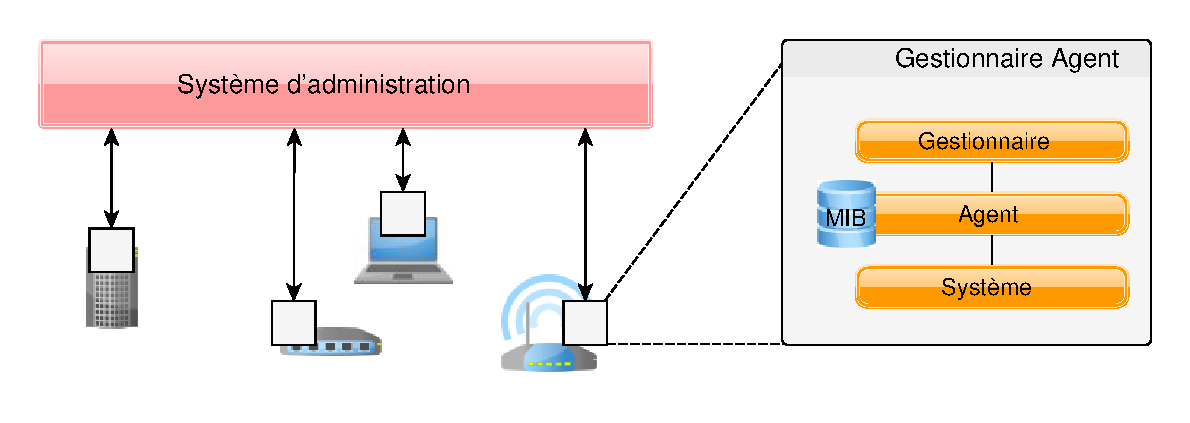
\includegraphics[width=.75\textwidth]{fig/rw-supervision-administration}
    \caption{Architecture d'un système classique d'administration}\label{fig:rw:supervision:administration}
\end{figure}

\subsubsection{Les données fournies les agents}
Il existe plusieurs structures abstraites de données dans le cadre des systèmes d'administrations. La structure la plus répandue reste la \textbf{structure hiérarchique}. La première apparition d'un tel modèle de donnée remonte à la spécification de SNMP~\cite{IETF:SNMP} qui décrit le concept de \textit{Management Information Base} (MIB)~\cite{IETF:MIB}. Une \textit{MIB} est une base d'information où les données sont regroupées sous forme d'arbre. Chaque information possède à l'intérieur de ce arbre un chemin unique (l'\textit{object identifier}) décrit par une suite de chiffres séparés de points. Par exemple, \verb|1.3.6.1.2.1.2.2.1.2| est le chemin décrivant le nom d'une interface réseau sur un dispositif (par exemple \textit{eth0} sur un système Linux). Et le sous-arbre \verb|1.3.6.1.2| (MIB-II~\cite{IETF:MIB-II}) contient toutes les informations concernant les informations réseaux du dispositif.

Par la suite, l'idée des structures hiérarchiques a été reprise pour créer les protocoles d'administrations plus récents : le modèle de données TR-069 (décrit dans le TR-106~\cite{BBF:tr106}) et le service de gestion de configuration (CMS) de UPnP-DM~\cite{UPnP:DMCMS}. Dans ces derniers, le modèle de donnée est décrit comme un système de fichier. Les \textit{instances} sont assimilables à des dossiers, et les \textit{feuilles} sont assimilables à des fichiers. Les nœuds ont ainsi un nom et un chemin unique vers la racine \enquote{/}. Tout comme leurs analogues, les \textit{instances} n'ont pas de valeurs associées alors que les \textit{feuilles} contiennent une donnée. Il existe plusieurs types d'\textit{instances} :
\begin{itemize}
    \item \textit{Unique} : Ce nœud peut contenir tout autre nœud. Il représente simplement un chemin intermédiaire d'un groupe de données.
    \item \textit{Multiple} : Ce nœud peut contenir plusieurs nœuds de type \textit{Instance}. Il permet de représenter une liste de nœuds de même structures.
    \item \textit{Instance} : Il représente l'élement de la liste définie par l'instance multiple. Son nom sera toujours un entier pour l'identifier parmi les autres instances. Ces nœuds ont pour vocation à être créés ou supprimés en fonctionnement.
\end{itemize}
\begin{figure}[ht]
    \centering
    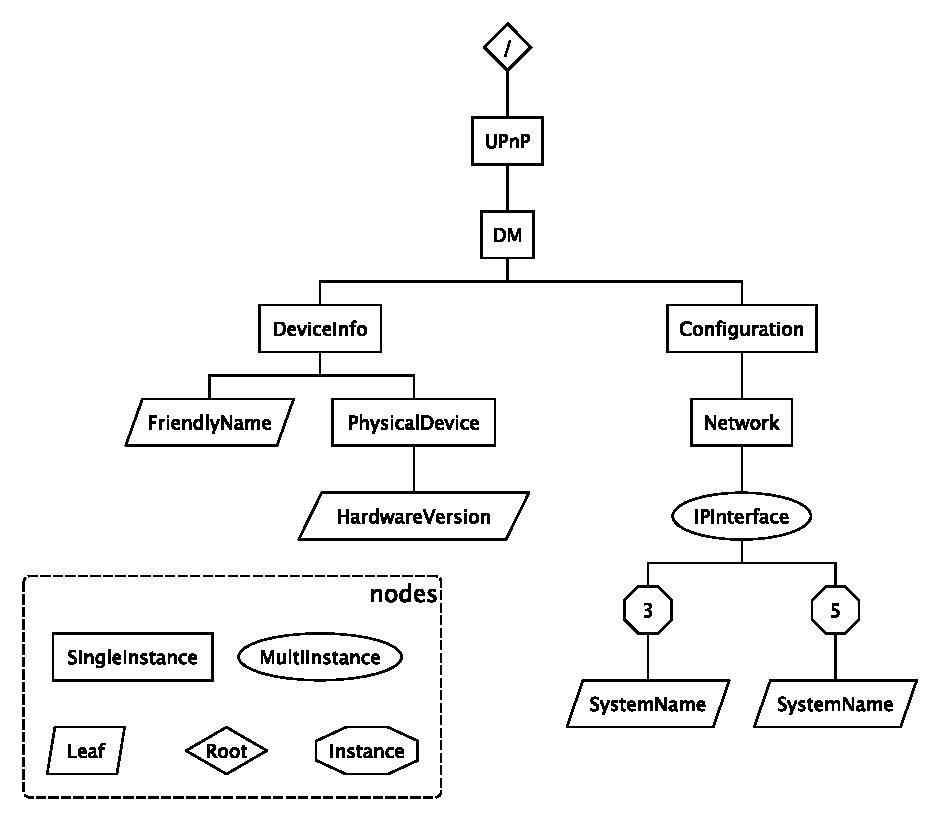
\includegraphics[width=.75\textwidth]{fig/rw-supervision-dmtree}
    \caption{Structure hiérarchique du modèle de données d'UPnP-DM}\label{fig:rw:supervision:dmtree}
\end{figure}

Un exemple de modèle de données de ce type de structure est présenté en figure~\ref{fig:rw:supervision:dmtree}. Désormais, une donnée est définie de manière unique, tout comme dans la MIB, grâce à son chemin complet. Dans le vocabulaire du domaine de l'administration, cette donnée est appelé \textit{paramètre}. Le \textit{chemin} d'un paramètre est la concaténation des noms des nœuds qui le sépare de la racine, avec pour séparateur \enquote{/} dans UPnP ou \enquote{.} dans TR-069. Voici quelques exemples de paramètres :
\begin{itemize}
\item \verb|/UPnP/DM/DeviceInfo/PhysicalDevice/HardwareVersion| permet de connaître la version du matériel du dispositif administré. 
\item \verb|/UPnP/DM/Configuration/Network/IPInterface/3/SystemName| est le nom d'une des interfaces réseaux (tout comme \verb|1.3.6.1.2.1.2.2.1.2| dans la MIB). En remplaçant \verb|/3/| par \verb|/5/|, cela concernera une autre interface réseau. Pour désigner toutes les instances d'un nœud multiple, la notation \verb|/#/| indique un numéro d'instance quelconque.
\end{itemize}

L'implémentation de l'agent permettra par la suite de pouvoir créer et remplir cette base d'information.

\begin{figure}[ht]
    \centering
    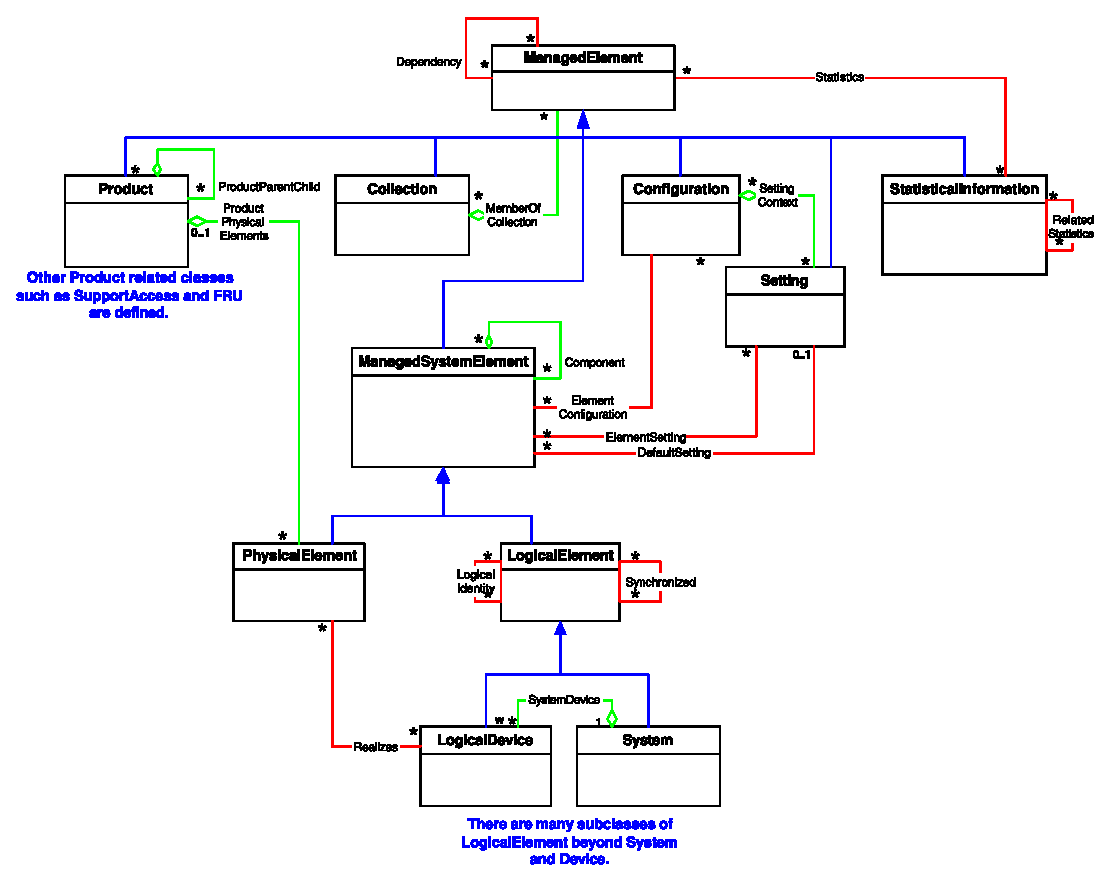
\includegraphics[width=.75\textwidth]{rw-supervision-cimcore}
    \caption{Modèle de classe de la partie \textit{Core} de \textit{CIM}}\label{fig:rw:supervision:cimcore}
\end{figure}
Toutefois, tous les modèles ne sont pas tous orientés sur la hiérarchie. Par exemple, la DMTF a adopté l'approche objet. En effet, dans les protocoles tels que WBEM~\cite{DMTF:WBEM} ou WS-MAN~\cite{DMTF:WS-MAN}, la fondation du modèle de données \textit{CIM} (\textit{Common Information Model})~\cite{DMTF:CIM} est décrite par un diagramme de classe UML comme présenté en figure~\ref{fig:rw:supervision:cimcore}. Ces protocoles sont notamment utilisé pour l'administration de web-services et applications entreprises. Nous pouvons remarquer la présence des différents concepts des structures précédentes avec le concept de \textit{Settings}, de \textit{ManagedElement}, et de \textit{Collection}. Plusieurs extensions standardisées existent pour modéliser les différents aspects des systèmes : Base de données, Dispositifs, Réseau, Sécurité, Utilisateur, Applications\dots{} Ainsi, le modèle des données sera un modèle d'objet respectant l'ensemble des spécifications et des extensions. L'inconvénient majeur d'un tel choix de méta-modèle restant la complexité de \textit{CIM} qui se trouve souvent réduite pour être applicable en pratique.

Le système se compose ainsi de multiples agents qui seront une représentation de chaque objet. Les objets du systèmes sont ainsi exposés à un service de gestion pour en fournir plusieurs propriétés. Nous pouvons noter que ce principe reste le même pour l'administration de modules Java dans le protocole JMX~\cite{Sun:JMX} où des objets particuliers (les \textit{MBean}) sont exposés et peuvent être consultés ou manipulés via ce protocole.

\subsubsection{Dynamisme des données}
Pour les différentes solutions présentés, les agents ont toujours trois modes principaux pour fournir des données permettant différentes dynamiques.
\begin{itemize}
	\item[\textbf{Consultation indirecte}: ] Ce fonctionnement est le plus simple. La donnée est stockée dans une base d'information quelconque. Au moment de la consultation, l'agent lit directement dans la base et renvoie l'information.
	\item[\textbf{Consultation active}: ] Au moment de l'appel de la données par l'utilisation via des primitives comme \enquote{\it get} sur le modèle de données, l'agent va effectuer le relevé actif de la donnée à la source. Par exemple, pour \textit{UPnP-DM}, plusieurs nœuds du modèle nécessitent de faire fonctionner une application en ligne de commande.
	\item[\textbf{Événement}: ] La plupart des systèmes d'administrations supportent un mécanisme de \textit{publish}/\textit{subscribe} permettant de créer des canaux d'événements. La création d'événement se fait à partir du changement de valeur d'un paramètre ou à la création d'instances.
\end{itemize}

Le problème majeur étant que la consultation et les canaux d'événements sont deux approches et deux mécanismes différents qui sont rarement intégrés.

\subsubsection{Le gestionnaire global}
Dans l'architecture présentée en figure~\ref{fig:rw:supervision:administration}, de multiples agents fournissent différentes informations selon les modèles présentés dans la section précédente. Le système d'administration se connecte aux différents agents afin de les gérer. Il sert à la fois d'interface à l'utilisateur que d'infrastructure de collecte et d'analyse. En effet, l'intégration des données ainsi que la vue globale du système s'y constituera.

Il est important de noter que ce système peut ne pas être centralisé pour mieux amortir la charge en la présence de grande quantités d'agents à administrer. Toutefois, il est important de voir que pour de l'administration de dispositifs des architectures centralisés peuvent suffir. Par exemple, pour l'administration de ses dispositifs, \textit{France Telecom} utilise un \textit{ACS} (serveur d'administration en TR-069) centralisé. En effet, la fréquence d'émission des données en fonctionnement normal se compte en jour pour chaque dispositif. Pour les 10 millions d'équipement à gérer, une capacité de 500 réceptions par seconde côté serveur est suffisante. Cette capacité est atteinte sur des \textit{ACS} récents tels que \textit{EDGE}~\cite{Motorola:EDGE} de \textit{Motorola} sur des serveurs de puissance moyenne.

Toutefois, plus l'usage le requiert, plus ce type d'architecture ne pourra supporter la charge des informations remontées. Plusieurs systèmes d'administrations supportent des structures décentralisées (principalement hiérarchiques) pour la gestion à plus grande échelle~\cite{Kessis:management}. La hiérarchie peut se découper par lieu géographique, ou par domaine d'activité. Dans le cadre des gestions par objets, le découpage par domaine permettra de répartir l'ensemble des agents par unité de traitement.

Nous venons de voir comment les systèmes d'administrations étaient structurés et notamment comment ces systèmes modélisent leurs données. La section suivante présente les capacités de traitements de ce type de systèmes.

\subsection{Possibles traitements de données}
Que ce soit au niveau de l'agent comme au niveau du gestionnaire global, les données peuvent être traitées. Cette section détaille les différents traitements possibles. Tout d'abord, nous verrons comment l'hétérogénéité des systèmes est traitée et comment l'intégration des multiples agents se fait. Par la suite nous verrons l'ajout de nœuds particuliers comme le calcul de statistique ou l'ajout de fonction tierces.

\subsubsection{L'hétérogénéité par la standardisation}
La standardisation est l'argument majeur des systèmes à grande échelles. Comme présenté précédemment, les protocoles d'administrations et la spécification des agents se fait autour de consortiums. Ainsi l'hétérogénéité des systèmes est gérée par le fait qu'il est supposé acquis que les standards soient respectés. Suivant les dispositifs observés, différents profils existent. Que ce soit pour les profils hiérarchiques ou à objet, des spécifications sont écrites pour décrire le modèle de données.

\begin{wraptable}{R}{7cm}
\centering
{\scriptsize
\begin{tabular}{cc}
\toprule
Profil & Spec. \\ \toprule
passerelle internet & TR-098 \\ \midrule
service de voix & TR-104 \\ \midrule
dispositifs & TR-106 \\ \midrule
décodeur tv & TR-135 \\ \midrule
service de stockage & TR-140 \\ \midrule
composants logiciels & TR-157 \\ \midrule
dispositifs génériques v.2 & TR-181 \\  \midrule
politiques d'accès aux services &  TR-196 \\ \midrule
femto cellule & TR-262 \\ \bottomrule
\end{tabular}}
\caption{Liste  des profils TR-069}\label{tab:rw:supervision:tr069dm}
\end{wraptable}
Il est notable que le nombre de spécification augmente énormément pour essayer d'amortir la grande hétérogénéité. Par exemple, dans le cadre de \textit{TR-069}, l'avantage étant que ce consortium couvre principalement l'usage des opérateurs télécoms, ainsi il existe seulement 9 profils principaux présentés en table~\ref{tab:rw:supervision:tr069dm}. Mais lorsque les domaines s'élargissent le nombre d'entités devient difficile à contrôler, comme dans CIM où le nombre de spécifications est de 16\footnote{Sachant que les spécifications CIM sont bien plus complexes et possèdent plus de classes.}, ou dans les MIB qui sont au nombre de 318 spécifiées par l'IETF.

De plus, ces spécifications ont plusieurs versions. Bien que la majeure partie soit rétro-compatible, certains profils subissent parfois des évolutions majeures. Par exemple, le TR-181 décrit les dispositifs génériques notamment en rassemblant les passerelles internets et les dispositifs communs auparavant décrit dans des profils séparés. 

Donc la gestion de l'hétérogénéité de fait par la description de profils de modèles. Toutefois, la standardisation amène plusieurs problèmes de complexité à maîtriser par les utilisateurs.

\subsubsection{Intégration de sources}
L'avantage principal d'utiliser des modèles standards est l'intégration des sources de données. En effet, comme chacune des entités du système répond à un profil pré-défini, il est possible de faire l'union des données par catégorie pour avoir toutes les entités répondants aux différents profils. Ainsi, les données sont naturellement intégrées dans un modèle commun, ce qui permet aux concepteurs de systèmes d'observations de fournir des fonctions très avancés sur des systèmes encore inconnus. De plus, plusieurs protocoles et standards peuvent être utilisés dans un même système, comme l'a proposé WBEM, dans lequel des objets SNMP, JMX et autres sont intégrés à un modèle commun CIM.

Une fois les données accessibles à un niveau fédérateur, il devient possible de traiter ces données afin de les corréler, ou former des alertes. Pour cela, les systèmes d'administrations ne fournissent pas tous les mêmes capacités. Par défaut, la seule capacité que peut fournir l'agent étant la récupération de son modèle de données (ou une sous-partie). Cependant, plusieurs systèmes permettent à l'utilisateur de définir des processus plus complexes pour permettre un traitement de plus haut niveau.

L'approche la plus utilisée étant le scripting. Le système d'observation fournit à l'utilisateur un langage \textbf{impératif} qui lui permettra de définir des routines. Par exemple, EDGE~\cite{Motorola:EDGE} fournit une interface \textit{Javascript}, et l'ACS d'Alcatel Lucent lui est adaptable avec des programmes \textit{Python}. Ces routines pourront par la suite être intégrées dans des réponses aux événements, dans des procédures de diagnostics ou de configuration.

Il est notable que dans les standards WBEM et WS-MAN, il est défini un langage \textbf{déclaratif} de manipulation de modèles CIM, le \textit{CQL} (\textit{CIM Query Language})~\cite{DMTF:CIM-QL}. Ce langage est très similaire à \textit{SQL} utilisé dans un cadre relationnel-objet. Dans sa spécifications, il permet toutes les fonctionalités d'\textit{SQL} (selection, projection, jointure, agrégation, imbriquation de requêtes). Il est aussi utilisé afin de permettre de faire des filtres plus précis sur les événements (en remplacement du langage par défaut étant \textit{XPath}). Il est intéressant de noter que le langage de définition de \textit{politiques de gestions} (routines événements-condition-action) peut être définies grâce à ce type de langage. Toutefois, il reste peu implémenté dans la pratique.

\subsubsection{Sur l'agent : statistiques et extension}
Dans chacune des solutions présentés, il existe des parties du modèle de donnée consacré à la présentation de statistiques. En effet, pour un paramètre dont la valeur représente une mesure, il peut être intéressant de fournir des extremums ou moyennes calculés à la volée. Plusieurs standardisations existent pour permettre un tel calcul sur une fenêtre de temps donnée (ou sur un nombre de relevé donné).

Tous les modèles présentés sont extensibles à volonté par les constructeurs des dispositifs. Par exemple sous UPnP-DM et TR-069, il est autorisé de rajouter des branches à l'arbre de données sous l'appellation \verb|X_{ORGANISATION}| (par exemple \verb|X_ORANGE_COM|). Ainsi, cela permet aux constructeurs de fournir des données non prévues dans les standards ou pour rajouter des fonctionalités de traitement.

\subsection{Synthèse}

\begin{table}[!ht]
\criteretabDonnee
    {Principalement structure \textbf{hiérarchique} sous forme de système de fichier. Quelques systèmes d'administration utilisent des modèles objets avec \textit{CIM}, mais reste difficile à maîtriser.}
    {Une donnée est identifié par son chemin complet. La sémantique est décrite par ce chemin. Pas de contraintes ou inférences exprimables.}
    {Le dynamisme est géré par le mode d'accès. Certaines données peuvent être notifiables. Les mécanismes d'interrogation sont séparés.}
\criteretabTraitement
    {Instantané et continu sur certaines données. Pas d'hybride possible vu que les procédés sont très séparés.}
    {Standardisation des modèles. Toutes les entités sont structurés dans le même formalisme. Intégration par union des données pour chaque profil.}
    {Appel de méthodes standardes pour récupérer un sous-arbre du modèle. Code impératif (scripting) principalement pour manipuler les données au niveau du gestionnaire. Utilisation de langage déclaratif (SQL ou XQuery) possibles.}
    {Projection, sélection et union principalement. Certains nœuds particuliers permettent de calculer des statistiques.}
\criteretabAdaptabilite
    {Pas d'adaptation spécifique car les dispositifs doivent implémenter des standards.}
    {Pas de perspectives métiers en dehors de la sélection sur les branches du modèle.}
    {Nœuds particuliers pour le calcul. Fonctions métiers intégrées dans le gestionnaire.}
    {Très efficace et utilisé pour gérer des parcs de millions de dispositifs.}
\caption{Synthèse des systèmes d'administration}\label{tab:rw:supervision:administration:synthese}
\end{table}

Le tableau~\ref{tab:rw:supervision:administration:synthese} résume l'ensemble de l'analyse qui a été porté aux systèmes d'administrations. L'ensemble permet effectivement beaucoup de fonctionnalité pour les utilisateurs. Le choix d'approches principales à base de standard fait que ces systèmes sont actuellement très répandus pour gérer des systèmes. Toutefois, le point le plus critique étant la gestion du dynamisme des données est faite dans des processus très différents rendant une supervision intégré difficile.